%\documentclass[mathserif]{beamer}
\documentclass[handout]{beamer}
%\usetheme{Goettingen}
\usetheme{Warsaw}
%\usetheme{Singapore}
%\usetheme{Frankfurt}
%\usetheme{Copenhagen}
%\usetheme{Szeged}
%\usetheme{Montpellier}
%\usetheme{CambridgeUS}
%\usecolortheme{}
%\setbeamercovered{transparent}
\usepackage[english, activeacute]{babel}
\usepackage[utf8]{inputenc}
\usepackage{amsmath, amssymb}
\usepackage{dsfont}
\usepackage{graphics}
\usepackage{cases}
\usepackage{graphicx}
\usepackage{pgf}
\usepackage{epsfig}
\usepackage{amssymb}
\usepackage{multirow}	
\usepackage{amstext}
\usepackage[ruled,vlined,lined]{algorithm2e}
\usepackage{amsmath}
\usepackage{epic}
\usepackage{epsfig}
\usepackage{fontenc}
\usepackage{framed,color}
\usepackage{palatino, url, multicol}
\usepackage{listings}
%\algsetup{indent=2em}


\vspace{-0.5cm}
\title{Directed Graphical Models}
\vspace{-0.5cm}
\author[Felipe Bravo Márquez]{\footnotesize
%\author{\footnotesize  
 \textcolor[rgb]{0.00,0.00,1.00}{Felipe José Bravo Márquez}} 
\date{ \today }




\begin{document}
\begin{frame}
\titlepage


\end{frame}


%%%%%%%%%%%%%%%%%%%%%%%%%%%


\begin{frame}{Directed Graphical Models}
\scriptsize{
\begin{itemize}
\item Probabilistic graphical models (PGMs) are a rich framework for encoding probability distributions over complex domains  \cite{koller2009probabilistic}.

\item In this class we will focus on directed graphical models (DGMs), which are one type of PGM.

\item Directed graphical models (DGMs) are a family of probability distributions that admit a compact parametrization that can be naturally described using a directed graph.

\item DGMs are also known as Bayesian networks.

\item Statistical inference for DGMs can be performed using frequentist or Bayesian methods, so it is misleading to call them Bayesian networks \cite{wasserman2013all}.



 
\end{itemize}



} 

\end{frame}


\begin{frame}{Directed Acyclic Graphs (DAGs)}
\scriptsize{
\begin{itemize}
\item A directed graph consists of a set of nodes with arrows between some nodes.


\item Graphs are useful for representing independence relations between variables.

\item More formally, a directed graph G consists of a set of vertices V and an edge set E of ordered pairs of
vertices.

\item For our purposes, each vertex corresponds to a random variable. 

\item If $(Y, X) \in E$  then there is an arrow pointing from Y to X. 

\begin{figure}[h!]
	\centering
	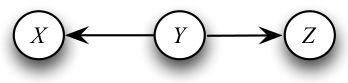
\includegraphics[scale=0.5]{pics/dag1.png}
	\caption{A directed graph with vertices $V = \{X, Y, Z\}$ and edges $E = \{(Y, X), (Y, Z)\}$.}
	\end{figure} 


 
\end{itemize}



} 

\end{frame}



\begin{frame}{Directed Acyclic Graphs (DAGs)}
\scriptsize{
\begin{itemize}
\item If an arrow connects two variables X and Y (in either direction) we say that X and Y are adjacent.


\item If there is an arrow from X to Y then X is a parent of Y and Y is a child of X.

\item The set of all parents of X is denoted by $\pi_{X}$ or $\pi(X)$.

\item A directed path between two variables is a set of arrows all pointing in the same direction linking one variable to the
other such as the chain shown below:

\begin{figure}[h!]
	\centering
	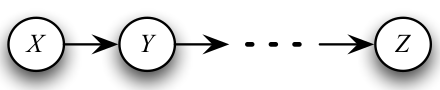
\includegraphics[scale=0.5]{pics/dag2.png}
	\caption{A chain graph with a directed path.}
	\end{figure} 

\item X is an ancestor of Y if there is a directed path from X to Y (or X = Y ).

\item We also say that Y is a descendant of X.
 
\end{itemize}



} 

\end{frame}

\begin{frame}{Directed Acyclic Graphs (DAGs)}
\scriptsize{
\begin{itemize}
\item A directed path that starts and ends at the same variable is called a cycle.

\item A directed graph is acyclic if it has no cycles. 

\item In this case we say that the graph is a directed
acyclic graph or DAG. 


\begin{figure}[h!]
	\centering
	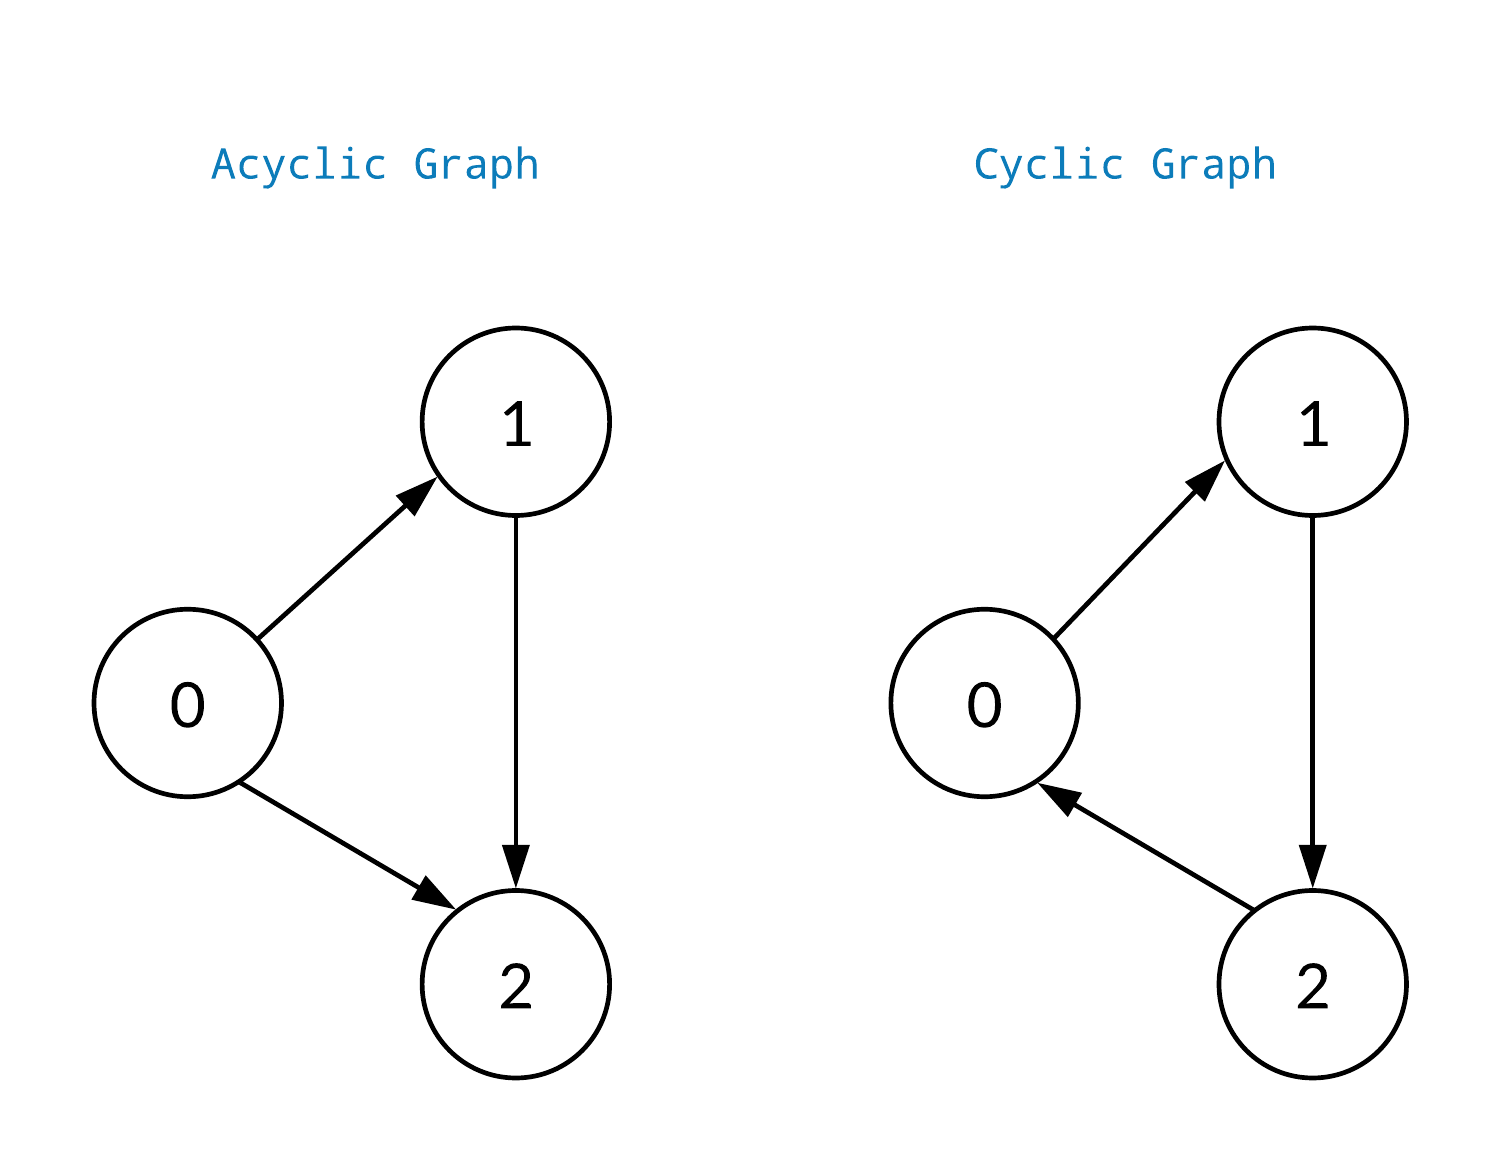
\includegraphics[scale=0.12]{pics/cycle.png}
	\end{figure} 



\item From now on, we only deal with directed acyclic graphs since it is very difficult to provide a coherent probability semantics over graphs with directed cycles.
 
\item For the remainder of this class we will use the terms Bayesian Network, directed graphical model (DGM) and directed acyclical graph (DAG) interchangeably. 
 
 
\end{itemize}



} 

\end{frame}


\begin{frame}{Probability and DAGs}
\scriptsize{
\begin{itemize}

\item An important concept we need to introduce to understand DAGs is the chain rule of probability.

\item For a set of random variables $X_1,\dots, X_n$ we can write the joint probability function $f(x_1,x_2,\dots, x_n)$ as 

\begin{displaymath}
f(x_1,x_2,\dots,x_n)=f(x_1)f(x_2|x_1)\dots f(x_n|x_{n-1},\dots,x_2,x_1).
 \end{displaymath}



\item A DAG is a distribution in which each factor on the right hand side depends only on a small number of ancestor variables $\pi(x)$. \cite{ermon_kuleshov}



\item Let $G$ be a DAG with vertices $V = (X_1 , \dots , X_d )$. 

\item If $P$ is a distribution for $V$ with probability function $f(x)$ (density or masss), we say that $G$ represents $P$ , if

\begin{displaymath}
 f(x) = \prod_{j=1}^d f(x_j| \pi_{x_j})
\end{displaymath}

where $\pi_{x_j}$ is the set of parent nodes of $X_j$



\end{itemize}



} 

\end{frame}

\begin{frame}{Probability and DAGs}
\scriptsize{
\begin{itemize}


\item The next figure shows a DAG with four variables.

\begin{figure}[h!]
	\centering
	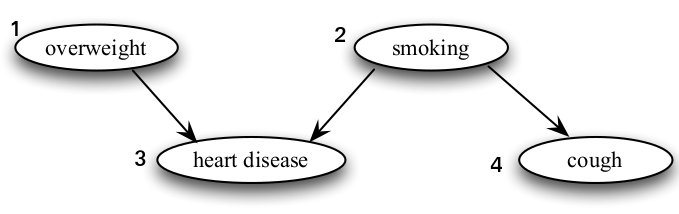
\includegraphics[scale=0.4]{pics/dag3.png}
	\end{figure} 



\item The probability function takes the following decomposition:

\item $f($overweight, smoking, heart disease, cough$) =$ \\    $f($overweight$) \times f($smoking$) \times f($heart, disease$|$ overweight, smoking$) \times f($cough$|$smoking$)$. 


\end{itemize}



} 

\end{frame}





\begin{frame}{Conditional Independence}
\scriptsize{
\begin{itemize}
\item Let $X$, $Y$ and $Z$ be random variables. 

\item $X$ and $Y$ are conditionally independent given $Z$, written $X \perp Y | Z$, if:

\begin{displaymath}
f(x, y|z) = f(x|z)f(y|z) 
\end{displaymath}


for all x, y and z.

\item Notice that $f$ can be either a density function for continous random variables or a probability mass function for discrete random variables.
 
\item Intuitively, this means that, once you know $Z$, $Y$ provides no extra information about $X$. 
 
\end{itemize}



} 

\end{frame}


\begin{frame}{An Example}
\scriptsize{
\begin{itemize}
\item The best way to understand DAGs is to imagine trying to model a situation in which causality plays a role.
\item And also our understanding of what is actually going on is
incomplete
\item So we need to describe things probabilistically. 

\item The following example is based on \cite{charniak1991bayesian}.

\item Eugene Charniak is a famous AI researcher who's got the following situation.

\item When he goes home at night, he wants to know if his family is home before trying the doors. 

\item Often when his wife leaves the house, she turns on an outdoor light. 

 
\end{itemize}



} 

\end{frame}



\begin{frame}{An Example}
\scriptsize{
\begin{itemize}

\item Eugene's wife can also turn on the outdoor light if she is expecting a guest.

\item Also, they have a female dog. 

\item When nobody is home, the dog is put in the back yard. 

\item The same is true if the dog has bowel troubles. 

\item Finally, if the dog is in the backyard, Eugene's will probably hear her barking 

\item The next slide shows a DAG encoding all the above causal relationships.

 
\end{itemize}



} 

\end{frame}


\begin{frame}{An Example}
\scriptsize{

\begin{figure}[h!]
	\centering
	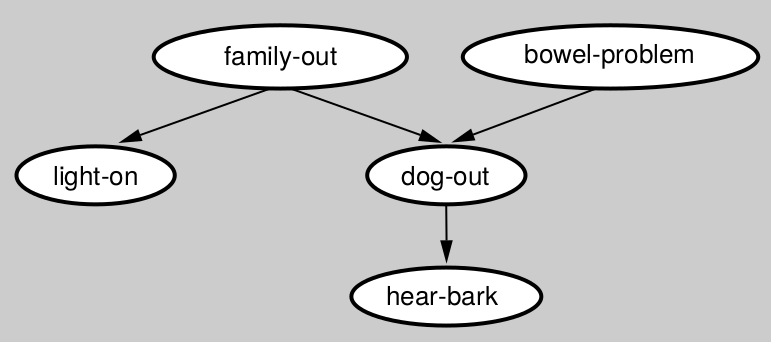
\includegraphics[scale=0.4]{pics/fodag.png}
	\end{figure} 

\begin{itemize}

\item The DAG can help to predict what will happen in a particular scenario (if his family goes out, the dog goes out) 
\item Or to infer causes from observed effects (if the light is on and the dog is out, then his family is probably out).



 
\end{itemize}



} 

\end{frame}


\begin{frame}{D-separation}
\scriptsize{
\begin{itemize}
\item sdsad

 
\end{itemize}



} 

\end{frame}


\begin{frame}{Plate Notation}
\scriptsize{
\begin{itemize}
\item sdsad

 
\end{itemize}



} 

\end{frame}



\begin{frame}{Estimation for DAGs}
\scriptsize{
\begin{itemize}
\item Two estimation questions arise in the context of DAGs. 
\item First, given a DAG $\mathcal{G}$ and data $d_1,\dots,d_n$ from a distribution $f$ consistent with $\mathcal{G}$, how do we estimate f?

\item Second, given data $d_1,\dots,d_n$ how do we estimate $\mathcal{G}$?

\item The first question is pure estimation while the second involves model selection.

\item These are very involved topics and are beyond the scope of this course.

\item We will just briefly mention the main ideas.

 
\end{itemize}



} 

\end{frame}


\begin{frame}{Estimation for DAGs}
\scriptsize{
\begin{itemize}

\item If we are doing frequentist inference, we typically use some parametric model $f(x|\pi_x;\theta_x)$ for each conditional density. 

\item The likelihood function is then

\begin{displaymath}
 \mathcal{L}(\theta) = \prod_{i=1}^nf(d_i;\theta) ) =  \prod_{i=1}^n\prod_{j=1}^mf(X_{ij}|\pi_j;\theta_j) 
\end{displaymath}

\item where $X_{ij}$ is the value of $X_j$ for the ith data point and j are the parameters for the-jth conditional density. 

\item We can then estimate the parameters by maximum likelihood.

\item On the other hand, if we want to perform Bayesian inference we must set priors for all our variables $X_1,\dots,X_m$ and estimate the posterior accordingly.

 
\end{itemize}



} 

\end{frame}

\begin{frame}{Estimation for DAGs}
\scriptsize{
\begin{itemize}

\item To estimate the structure of the DAG itself, we could fit every possible DAG
using maximum likelihood and use AIC (or some other method) to choose a
DAG. 

\item However, there are many possible DAGs so we would need much data
for such a method to be reliable.

\item Also, searching through all possible DAGs is a serious computational challenge. 

\item Producing a valid, accurate confidence set for the DAG structure would require astronomical sample sizes. 

\item If prior information is available about part of the DAG structure, the computational and statistical problems are at least partly ameliorated \cite{wasserman2013all}.

 
\end{itemize}



} 

\end{frame}


\begin{frame}{Conclusions}
\scriptsize{

\begin{itemize}
\item Blabla
\end{itemize}


} 
\end{frame}


%%%%%%%%%%%%%%%%%%%%%%%%%%%
\begin{frame}[allowframebreaks]\scriptsize
\frametitle{References}
\bibliography{bio}
\bibliographystyle{apalike}
%\bibliographystyle{flexbib}
\end{frame}  









%%%%%%%%%%%%%%%%%%%%%%%%%%%

\end{document}
